\documentclass{../../../oss-ap12ibhl}

\begin{document}
\genheader
\gentitle{16}{MODERN PHYSICS}

\begin{questions}

  \question Two blocks of different sizes and masses float in a tray of water.
  Each block is half submerged, as shown in the figure. Water has a density of
  \SI{1000}{\kilo\gram\per\metre^3}. What can be concluded about the
  densities of the two blocks?
    

  % THIS TAKEN FROM THE 2005 AP PHYSICS B EXAM FREE-RESPPONSE QUESTION #7
  \uplevel{
    \centering
    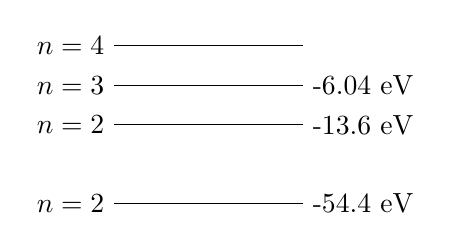
\begin{tikzpicture}[yscale=.5,xscale=.8]
      \draw(0, 0)--(3, 0) node[pos=0,left]{$n=4$};
      \draw(0,-1)--(3,-1) node[pos=0,left]{$n=3$} node[right]{-6.04 eV};
      \draw(0,-2)--(3,-2) node[pos=0,left]{$n=2$} node[right]{-13.6 eV};
      \draw(0,-4)--(3,-4) node[pos=0,left]{$n=2$} node[right]{-54.4 eV};
    \end{tikzpicture}
    
    \underline{Note:} Energy levels not drawn to scale.
  }

  \question The diagram above shows the lowest four discrete energy levels of an
  atom. An electron in the $n=4$ state makes a transition to the $n=2$ state,
  emitting a photon of wavelength \SI{121.9}{\nano\metre}.
  \begin{parts}
    \part Calculate the energy level of the $n=4$ state.
    \part Calculate the momentum of the photon.

    \uplevel{
      The photon is then incident on a silver surface in a photoelectric
      experiment, and the surface emits an electron with \underline{maximum}
      possible kinetic energy. The work function of silver is 4.7 eV.
    }

    \part Calculate the kinetic energy, in eV, of the emitted electron.
    \part Determine the stopping potential for the emitted electron.
  \end{parts}
  \newpage
  
  % THIS TAKEN FROM THE 2012 AP PHYSICS B EXAM FREE-RESPPONSE QUESTION #7
  \question The momentum of a particular proton is
  \SI{5.5e-20}{\kilo\gram\metre\per\second}. Relativistic effects can be
  ignored throughout this question.
  \begin{parts}
    \part Calculate the de Broglie wavelength of the proton.
    \part Calculate the kinetic energy of the proton.
    \uplevel{
      The proton is directed toward a very distant stationary uranium nucleus,
      $^{235}_{92}\text{U}$. The proton reaches a distance $D$ from the center of
      the nucleus and then reverses direction. Assume that the nucleus is heavy
      enough to remain stationary during the interaction.
    }
    \part Calculate the value of $D$.
    \part After the proton has moved away, the $^{235}_{92}\text{U}$ nucleus
    spontaneously fissions into $^{148}_{57}\text{La}$ and $^{84}_{35}\text{Br}$,
    along  with three neutrons. As a result, \SI{2.5e-11}{\joule} of energy is
    released. Indicate whether the mass of the nucleus is greater or less than
    the mass of the fission products. Calculate the mass difference.

    \vspace{.1in}
    \underline{\hspace{.3in}} Greater\hspace{.2in}
    \underline{\hspace{.3in}} Less
  \end{parts}
  \newpage

  \uplevel{
    \cpic{.6}{tube}
  }
  \question The apparatus shown above is used in determining the work function
  of a particular metal using the photoelectric effect. The experiment is set up
  with an ammeter A and a variable power supply. A light source that emits
  photons of frequency \SI{7.5e14}{\hertz} is used. The emf e provided by the
  power supply is slowly increased from zero until the ammeter shows that the
  current between the collector and metal emitter is zero. The magnitude of the
  emf is \SI{.65}{\volt} when the current becomes zero.
  \begin{parts}
    \part Determine the wavelength of the incident photons.
    \part Calculate the work function of the metal.
    \part Calculate the minimum frequency of light at which electrons would be
    emitted.
    \part If the power per unit area (intensity) of the incident light is
    increased and the wavelength stays the same, does the magnitude of the emf
    needed to stop the current increase, decrease, or remain the same? Justify
    your answer.

    \vspace{.1in}
    \underline{\hspace{.3in}}Increases\vspace{.2in}
    \underline{\hspace{.3in}}Decreases\vspace{.2in}
    \underline{\hspace{.3in}}Remains the same

    \vspace{.1in}
    
    \part If the wavelength of light is decreased while the power per unit
    area (intensity) of the incident light stays the same, does the number of
    electrons emitted from the metal surface per unit time increase, decrease,
    or remain the same? (Assume that the light is initially above the threshold
    frequency.) Justify your answer.

    \vspace{.1in}
    \underline{\hspace{.3in}}Increases\vspace{.2in}
    \underline{\hspace{.3in}}Decreases\vspace{.2in}
    \underline{\hspace{.3in}}Remains the same
  \end{parts}
  \newpage

  % THIS TAKEN FROM THE 2003 AP PHYSICS B EXAM FREE-RESPPONSE QUESTION #7
  \uplevel{
    \cpic{.65}{photons}
  }
  \question A photon of wavelength \SI{2.0e-11}{\metre} strikes a free electron
  of mass $m_e$ that is initially at rest, as shown above left. After the
  collision, the photon is shifted in wavelength by an amount
  $\Delta\lambda=2h/m_ec$, and reversed in direction, as shown above right.
  \begin{parts}
    \part Determine the energy in joules of the incident photon.
    \part Determine the magnitude of the momentum of the incident photon.
    \part Indicate below whether the photon wavelength is increased or
    decreased by the interaction. Explain your reasoning.
    \part Determine the magnitude of the momentum acquired by the electron.
  \end{parts}
  \newpage
  
  \question Energy-level diagrams for atoms that comprise a helium-neon laser
  are given above. As indicated on the left, the helium atom is excited by an
  electrical discharge and an electron jumps from energy level $E_0$ to energy
  level $E_2$. The helium atom (atomic mass 4) then collides inelastically with
  a neon atom (atomic mass 20), and the helium atom falls to the ground state,
  giving the neon atom enough energy to raise an electron from $E_0'$ to $E_2'$.
  The laser emits light when an electron in the neon atom falls from energy
  level $E_2'$ to energy level $E_1'$.
  \begin{parts}
    \part Calculate the minimum speed the helium atom must have in order to
    raise the neon electron from $E_0'$ to $E_2'$.
    
    \part Calculate the DeBroglie wavelength of the helium atom when it has the
    speed determined in (a).
    
    \part The excited neon electron then falls from $E_2'$ to $E_1'$ and emits
    a photon of laser light. Calculate the wavelength of this light.
    
    \part This laser light is now used to repair a detached retina in a
    patient's eye. The laser puts out pulses of length \SI{20e-3}{\second} that
    average \SI{.50}{\watt} output per pulse. How many photons does each pulse
    contain?
  \end{parts}
\end{questions}
\end{document}
